%        File: inlevering2.tex
%     Created: Thu Sep 26 05:00 PM 2013 C
% Last Change: Thu Sep 26 05:00 PM 2013 C
%

\documentclass[a4paper]{article}
\usepackage{hyperref}
\usepackage{graphicx}
\begin{document}
\title{TOD/DAT Innlevering 2}
\author{Paul Grant}
\date{\today}
\maketitle

\section*{Oppgave 1}{
  \subsection*{DRAM vs SRAM}{
    There are two types of RAM, static and dynamic. What makes these different is how they hold data. DRAM requires the data to be refreshed periodically for the data to stay in the memory. SRAM on the other hand doesn't need to be refreshed and the memory remains inside the transistors even if the power supply is cut off. SRAM is much more desirable than DRAM because it takes less power to use as well as being faster and does not have problems with losing data.//DRAM is cheaper than SRAM. This leads to DRAM being used in main memory (hard drives) and SRAM being used as cache memory (RAM).
  }
}
\section*{Oppgave 2}{
  \subsection*{Two's Complement}{
    This is a mathematical operation on binary numbers, as well as a binary signed number representation based on this operation. Its wide use in computing makes it the most important example of a radix complement.\\\\
    The two's complement of a N-bit number is defined as the complement with respect to $2^n$, in other words the result of subtracting the number from $2^n$. This is also equivalent to taking the ones' complement and then adding one, since the sum of a number and its ones' complement is all 1 bits. The two's complement of a number behaves like the negative of the original number in most arithmetic, and positive and negative numbers can coexist in a natural way.\\\\
    The two's-complement system has the advantage that the fundamental arithmetic operations of addition, subtraction, and multiplication are identical to those for unsigned binary numbers (as long as the inputs are represented in the same number of bits and any overflow beyond those bits is discarded from the result). This property makes the system both simpler to implement and capable of easily handling higher precision arithmetic. Also, zero has only a single representation, obviating the subtleties associated with negative zero, which exists in ones'-complement systems (
    \url{http://en.wikipedia.org/wiki/Two%27s_complement}).\\\\
34+32\\\\00100010\\+\\00100000\\=\\01000010\\\\
34-32\\\\00100010\\-\\00100000\\=\\00000010\\\\
32+-32\\\\00100010\\+\\11100000\\=\\00000010\\\\
34--32\\\\00100010\\-\\11100000\\=\\01000010\\\\
        }
    }
}
\section*{Oppgave 3}{
  \subsection*{Explanation of a Two-Set Associative Mapping Example:}
  This type of cache uses the least significant bits of the memory location's index as the index for the cache memeory, and to have two entries for each index. The benefit of this scheme is that the tags stored in the cache do not have to include the part of the main memory address which is implied by the cache memory's index (as shown in the right had portion of the example).
    

\section*{Oppgave 4}
  \subsection*{A) the AND}
    \begin{center}
      \begin{tabular}{| l | c | r | }
        \hline
        \hline A & B \\ \hline
        \hline T & T & T\\ \hline
        \hline T & F & T\\ \hline
        \hline F & F & T\\ \hline
        \hline F & T & F \\ \hline
        \hline

        \hline
        \hline A & B \\ \hline
        \hline 0 & 0 & 1\\  \hline
        \hline 0 & 1 & 1\\ \hline
        \hline 1 & 0 & 1\\ \hline
        \hline 1 & 1 & 0\\ \hline
        \hline

      \end{tabular}
    \end{center}
      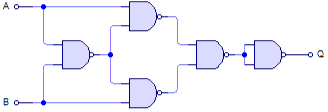
\includegraphics{XNOR_Using_NAND.png}
  \subsection*{B) the NOR}
    \begin{center}
      \begin{tabular}{|l|c|r|}
        \hline
        \hline A & B \\ \hline
        \hline T & T & T\\ \hline
        \hline T & F & F\\ \hline
        \hline F & F & F\\ \hline
        \hline F & T & F \\ \hline
        \hline
        
        \hline
        \hline A & B \\ \hline
        \hline 0 & 0 & 1\\ \hline
        \hline 0 & 1 & 0\\ \hline
        \hline 1 & 0 & 0\\ \hline
        \hline 1 & 1 & 0\\ \hline
        \hline
      \end{tabular}
    \end{center}
    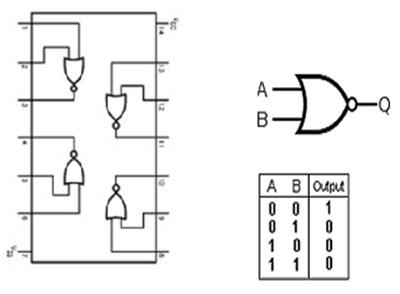
\includegraphics[scale=0.5]
    {Understanding-NOR-Gate(CD4001).jpg}

\end{document}


